\section{rTisane study materials} \label{appendix:summativeEvaluation} 

What follows are materials for the summative evaluation lab study, as described
in~\autoref{sec:summativeEval}. Phase 1 and each task labeled \textbf{Without \rTisane}
were in an editable word processing document shared with the participant. Each
task labeled \textbf{With \rTisane} was in an editable R Markdown file open in RStudio.
Participants edited the R Markdown files via remote control. 

\clearpage 
\section*{Phase 1: Warm up}
Scenario: You are a census researcher leading a team that investigates how an
individual’s background and demographic factors influence income. Your
motivating research question is \textit{``What aspects of an individual’s background and
demographics are associated with income after they have graduated from high
school?''}

\subsection*{Warm up}

What are your initial ideas about what factors influence income among adults?
Summarize your ideas in a \textbf{conceptual model}. A conceptual model specifies the
factors you know or hypothesize influence an outcome, what factors you think do
not influence an outcome, and how those factors might interact to give rise to
the outcome. 

For example, a conceptual model for plant growth might communicate
the following: Sunlight influences plant growth. Water influences plant growth.
Both sunlight and water are necessary for plant growth. Plant-owner love
influences plant growth because love influences plant placement, which might
influence sunlight. You might also express the above conceptual model as

\begin{figure}[H]
    \centering
    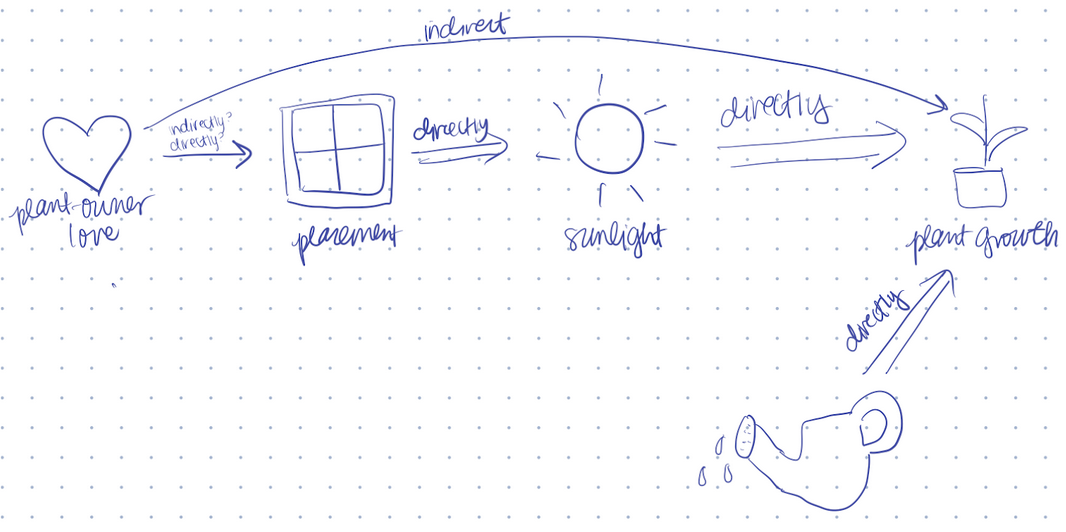
\includegraphics[width=.85\linewidth]{tisane/figures/example-conceptual-model.png}
    % \label{fig:figureConceptualModelsDisambiguation}
\end{figure}

1. Spend approximately 5 minutes to express your conceptual model. Consider
providing (i) a list of relationships between variables of the form ``Variable'',
``relationship'', ``Variable'' (e.g., ``Plant owner love, causes, plant growth'') OR
(ii) a diagram with variables and relationships between them clearly labeled,
similar to the above example diagram. Feel free to write or draw below. Here is
a canvas in case you prefer. 

\clearpage
\section*{Phase 2: Express conceptual models, Without \rTisane}
Your team is able to collect data about the below variables. The data that your team has collected can be found here. 
\begin{itemize}
    \item \textbf{Age} (continuous)
    \item \textbf{Race} (unordered categories)
    \begin{itemize}
        \item 5 categories:White, Black/African American, American Indian or Alaska Native, Asian or Pacific Islander, Mixed Race
    \end{itemize}
    \item \textbf{Highest Education Completed} (ordered categories)
    \begin{itemize}
        \item 5 categories: Grade 12, 1 year of college, 2 years of college, 4 years of college, 5+ years of colleges
    \end{itemize}
    \item \textbf{Current Employment Status} (unordered categories)
	\begin{itemize}
        \item 3 categories: N/A, Works for wage, Self-employed
    \end{itemize}
    \item \textbf{Sex} (unordered categories)
    \begin{itemize}
        \item 2 categories: Male, Female
    \end{itemize}
    \item \textbf{Income} (continuous)
\end{itemize}

Express a conceptual model including only the variables you and your team have
access to. Feel free to write or draw below. Here is a canvas in case you
prefer. 


% \subsubsection{With \rTisane}
% Make and add to PDF separately
\clearpage\thispagestyle{empty}\mbox{}\clearpage 

\section*{Phase 3: Implement statistical models, Without \rTisane}
\begin{enumerate}
    \item Relying on your conceptual model alone, implement a statistical model that
    assesses the influence of variables you believe to be important (in the context
    of additional potentially influential factors) on income.

    You are welcome to use any tools you would like. Please just make sure to share
    your screen. 

    \item Summarize the results of your analysis below.
\end{enumerate}

% \section*{Phase 3: Implement statistical models, With \rTisane}
% Make and add to PDF separately